\section{Segmenting Timeseries Using the DISCO software}
\label{sec:segmenting_timeseries}
DISCO is a comprehensive (we hope) software for automatically segmenting cells in trap like devices and inspecting/editing the result. The processing is done through a combination of a matlab script, which is run cell by cell, and a collection of GUI's. We have found that this combination allows people to customise their personal work flows and allows the software to be easily updated and maintained. The standard work flow is:
\begin{enumerate}
	\item The user points the software to the images that make up the experiment and provides some basic information about the experiment.
	\item The user checks the identification of traps in the images and sets a number of parameters, mostly by GUI.
	\item The software uses a \textbf{cellVision Model} and \textbf{cellMorphology Model} to automatically identify and track cells in the images.
	\item The user can at this stage check and edit the automated cell identification and tracking and select cells to exclude from the data extraction.
	\item The software extracts data for the selected cells which can be used in analysis.
\end{enumerate}
\begin{figure}
\centering
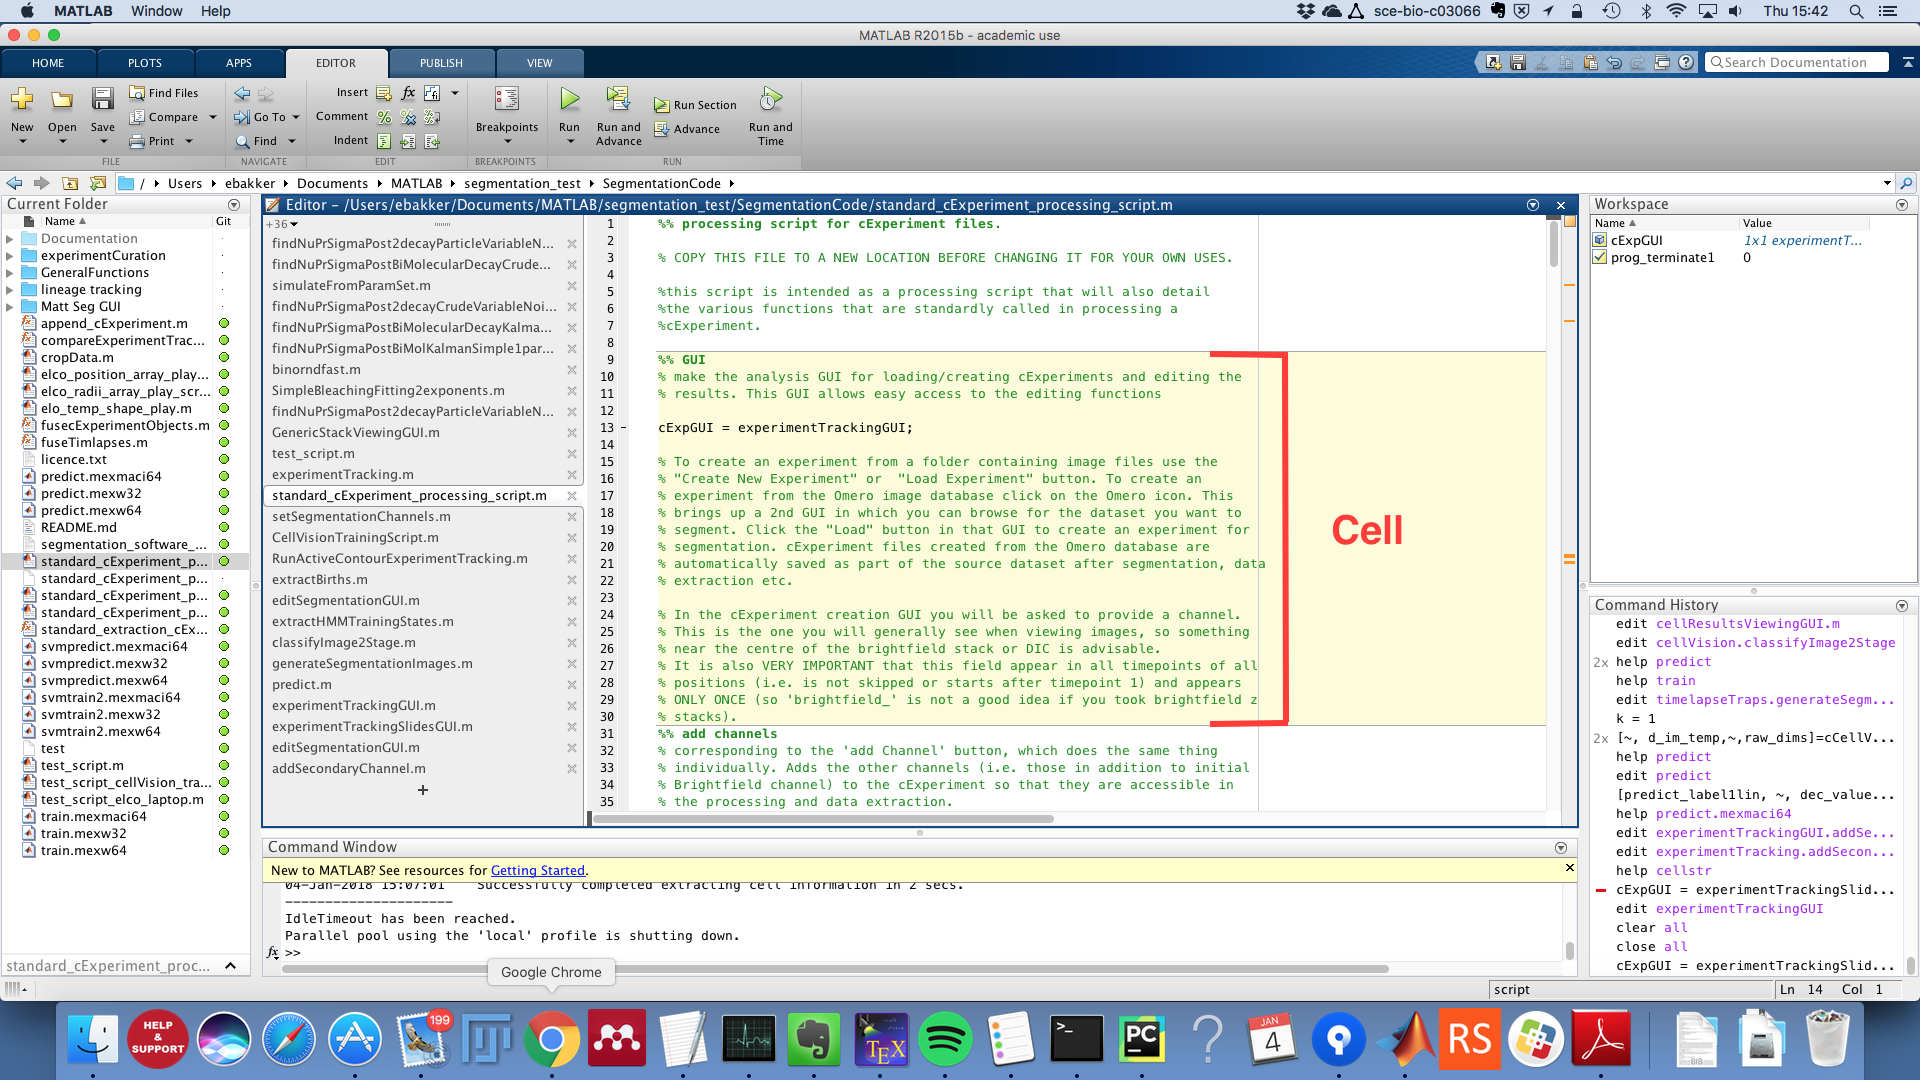
\includegraphics[width=1\linewidth]{documentation_images/standard_script_screen}
\caption[Screen-shot of the standard processing script.]{Screen-shot of the standard processing script. The script is broken into cells (indicated) by the \texttt{ $\% \%$} characters. Each cell contains some code and a description of what the code does, or why you would want to do it (green text). The highlighted (yellow) cell can be run by pressing \texttt{cmd Enter} for Mac and \texttt{ctrl Enter} for windows.}
\label{fig:standard_script_screen}
\end{figure}
\begin{figure}
\centering
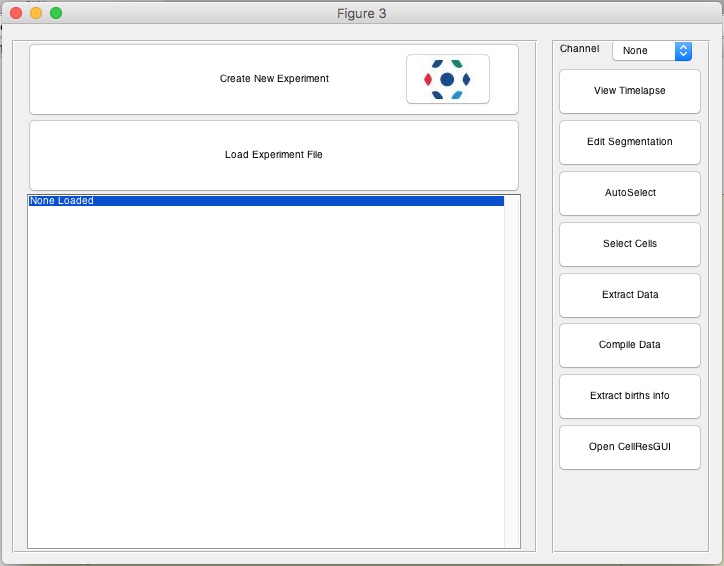
\includegraphics[width=0.5\linewidth]{documentation_images/experimentTrackingGUI}
\caption[Experiment tracking GUI]{Experiment tracking GUI. This is the primary GUI used in processing experiments. The buttons on the left, are for creating the experiment. The selection screen below is for selecting which positions to process and the buttons on the right are for checking and editing the result of the automated segmentation. By pressing 'h' one can open the help of the GUI.(Note: the colourful Omero Button to the right of Create New Experiment will only appear if you have the Omero software installed and is not necessary for processing experiments.)}
\label{fig:experimentTrackingGUI}
\end{figure}


To begin open the script called \texttt{standard\_cExperiment\_processing\_script.m}\footnote{in time you will find you want to change parts of this script to suit your own workflow. At this stage, copy the script with a new name and edit this version}; you should see something like the screen shot shown in figure \ref{fig:standard_script_screen}.\\
Run the first cell and a GUI, like that shown in figure \ref{fig:experimentTrackingGUI}, should open. This is the primary GUI for processing the software, and is used in combination with the script to process the experiment. By pressing 'h' one can see a help dialogue on all the buttons of the GUI (in general, 'h' will open a help dialogue for GUI's).\\
To start, press the top left button labelled 'Create New Experiment'. This will open a dialogue by which you point the software at the images you wish to process. The software has been designed for the Swain lab and our image storage structure, which is a top level folder containing one folder for each position imaged during the experiment, with each position folder containing the images for that position. At this stage one needs to select the folder \textbf{containing} the position folders. To read about how to get images stored in another way into the correct configuration using ImageJ (or FIJI) see section \ref{sec:other_systems}.\\
Now the experiment has been created, the positions can be viewed by pressing the 'View Timelapse' button (the position shown will be the topmost one highlighted on the left). Highlight all the positions you wish to process in the menu on the left and then return to the script. You will now need to run each of the cells in turn until you finally run the cell entitled \texttt{Actual long run (Elco standard extraction); run when happy with all the rest!}. This cell will commence the segmentation and data extraction of all the positions. 

\subsection{Notes and pointers:}
\begin{enumerate}
\item Depending on the length the experiment and the number of position, this last run may take a day or more. Most users run these overnight.
\item The code is parallelised in various places for speed. By default, matlab will use all available cores, which may be frustrating if you want to do other stuff in the meanwhile. You can get matlab to use only some of your cores using the \texttt{parpool} command before starting the analysis.
\end{enumerate}

\subsection{Checking and editing the result}
Once the automated segmentation has finished, one can inspect and edit the result in various ways using the buttons on the right of the experiment tracking GUI. By pressing 'h' when the experiment tracking GUI is the focus one can see a brief description of each GUI. When any of the GUI's are open one can get a fuller description by again pressing 'h'. 

\subsection{Accessing the Data}
When you are happy with the result, you will want to look at the extracted data. For the DISCO software, this takes the form of numerous statistics extracted for each of the selected channels for each of the selected cells. To see this go to the command line and type \texttt{cExperiment.cellInf}\footnote{If this is a new instance of matlab you will need to run the first cell of the script again to open the GUI, load the experiment and then run \texttt{cExpGUI.cExperiment.cellInf}}. Each entry in the structure array is a channel, each field is a statistic and each row is the value of that statistic over time for a particular cell. These are stored as sparse arrays, so when you find your desired channel and statistic it is best to copy it to the workspace and run \texttt{full(array\_name)} to make it a normal array. \\
To see a description of how each statistic was calculated type \texttt{help extractCellDataStandardParfor}.

\subsection{Diagnosing Poor Performance}
If the automated segmentation is performing badly, there are a number of things you can try to improve it. The problem is most likely either due to the cellVision model or the active contour parameters.
\subsubsection{cellVision model} You have inspected this as part of the standard script in the section titled \texttt{inspect decision image}.One can also see more details of the celLVision output by setting the parameter\\
 \texttt{cExperiment.ActiveContourParameters.ActiveContour.visualise = 4} \\
and running the processing on the first position. If the decision image is not dark and the centres of the cells and bright elsewhere then there is something wrong. You can try changing the channels used for the segmentation by running \texttt{cExperiment.setSegmentationChannels}, but if this fails you will need to retrain the cellVision model. It should be noted that the software is generally pretty robust, and retraining should only be necessary if you are using a new imaging modality or a new microscope. If neither of these is the case, you are most likely doing something wrong and it is probably worth contacting the authors or the swain lab (preferably the swain lab) before retraining the cellVision model.
\subsubsection{Active Contour Parameters}
There are various active contour parameters that can also be played with if the segmentation is not working well. These are stored in various substructures of the structure \texttt{cExperiment.ActiveContourParameters}, and I will try and describe the main ones and their effect here.
\begin{description}
	\item[TrapDetection] This is the set of parameters used for detecting the trap. If, when you run the software with \texttt{visualise = 4} as described above, the traps are not well blotted out (i.e. either too much or too litte blotting) then you need to change parameters here. One can try changing the channel, and can use negative channel indices to invert the channel. Try and pick a channel with a clear white trap on a black halo.
	\item[ActiveContour.alpha] This is the shape punishing term applied to new cells. If new cells are don't pay much attention to the image (i.e. are always a similar shape regardless of the image) and are a bit small make this parameter smaller. If new cells are very irregular shapes make this parameter larger.
	\item[ActiveContour.beta] This controls how much cells are constrained to be the same shape over time. If cells are too rigid (i.e. don't change shape in the way the images suggest) make this parameter smaller. If they change shape too much, make this parameter larger. One can also make this parameter larger if tracking often breaks.
	\item[ActiveContour.inflation\_weight] controls the force that expands cells. If the cells detected are too small, increase this. If they are too large, decrease this (note you should probably try changing alpha first).
	\item[CrossCorrelation.ThresholdCellProbability] this is the cell probability below which a cell will be discarded as `not being a real cell'. If a lot of cells are being discarded (as indicated by the `cells dicarded: ...' text when the software is running) the this is probably too high and should be turned down. If the software persists in keeping cells that don't `look good', then this is too low and should be increased.
\end{description}

If playing with these parameters does not solve the problem, feel free to contact a member of the swain lab for advice in improving performance.

\subsection{FAQ's}

\textbf{Why do you ask fo the pixel size when creating the experiment?}
The pixel size is used to determine whether an image has to be scaled to fit with the images used to train the software before processing. For example, our standard cellVision model was trained with 60x image (0.263 \microm pixels for our microscope), so if we want to segment 100x images (0.158 \microm pixels) the images need to be down sampled by a factor of $0.6$ .\\
The amount of down sampling required is determined by the software by comparing the pixel size submitted when the experiment is created and the pixel size of the experiment used to train the cellVision model. This is done when the traps are selected: the point at which the cellVision and the experiment are committed to each other.

\textbf{Why do I have to turn my traps to the left?}
This isn't strictly necessary if you are training a new cellVision model, but it was the orientation in which the first cellVision model was trained and has therefore become our convention. It is easier to share cellVision models between experiments if this convention is maintained.
